\section{Polar form}
\begin{itemize}
	\item $P=(r,\theta)$
	\item $r=f(\theta)$
\end{itemize}

\section{Converting between different forms of coordinates}
\subsection{Polar to Cartesian form}
\begin{itemize}
	\item $x=r\cos\theta$
	\item $y=r\sin\theta$
\end{itemize}
\subsection{Cartesian to polar form}
\begin{itemize}
	\item $r=\sqrt{x^2+y^2}$
	\item $\tan\theta=\dfrac{y}{x}$
\end{itemize}


\section{Sketching curves for polar equations}
\begin{enumerate}
	\item Plot points
	\item Consider symmetry
	\item Convert to Cartesian form
\end{enumerate}

\subsection{Testing for symmetry}
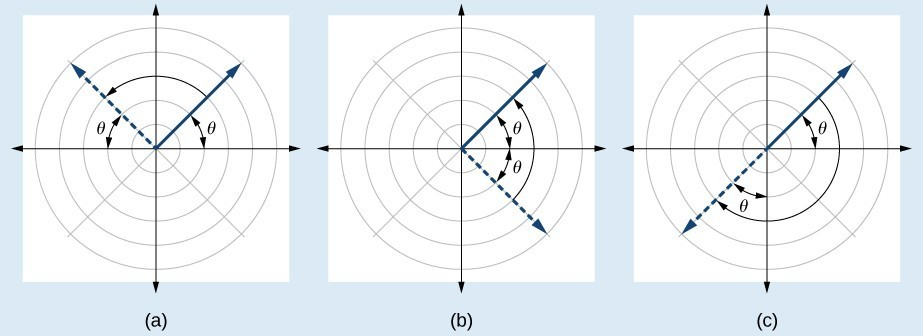
\includegraphics[width=0.5\textwidth]{symmetry_polar}
\begin{itemize}
	\item Symmetry about $\theta=0$ / $x$-axis: $f(\theta)=f(-\theta)$
	\item Symmetry about $\theta=\dfrac{\pi}{2}$ / $y$-axis: $f(\theta)=f(\pi-\theta)$
	\item Symmetry about pole / origin: $f(\theta)=f(\pi+\theta)$ / replacing $(r,\theta)$ with $(-r,
	\theta)$ gives an equivalent equation
\end{itemize}


\subsection{Circle polar form}
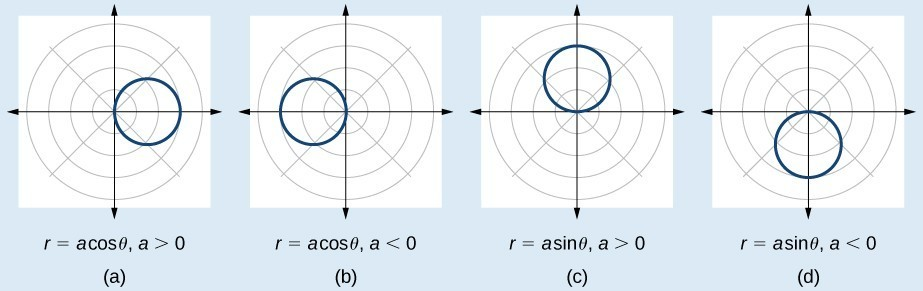
\includegraphics[width=0.7\textwidth]{circle_polar}

\subsection{Polar form of lines}
\begin{itemize}
	\item $\theta=a$: ray from origin
	\item $r\cos\theta=a$: equivalent to $x=a$
	\item $r\sin\theta=a$: equivalent to $y=a$
\end{itemize}

\subsection{Cardioids shape}
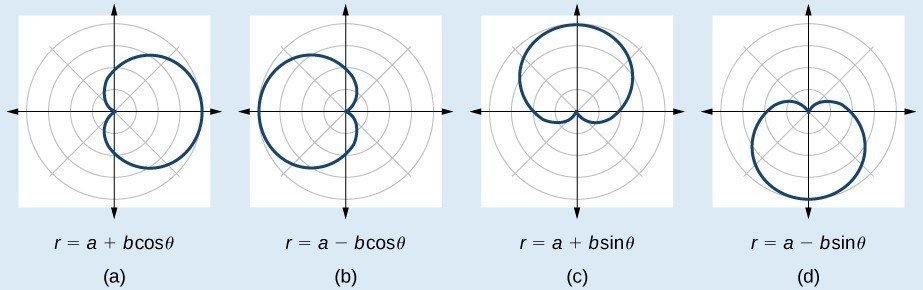
\includegraphics[width=0.7\textwidth]{cardioid_polar}
\subsection{Lima con shape}
\textbf{One-loop Lima con}\\
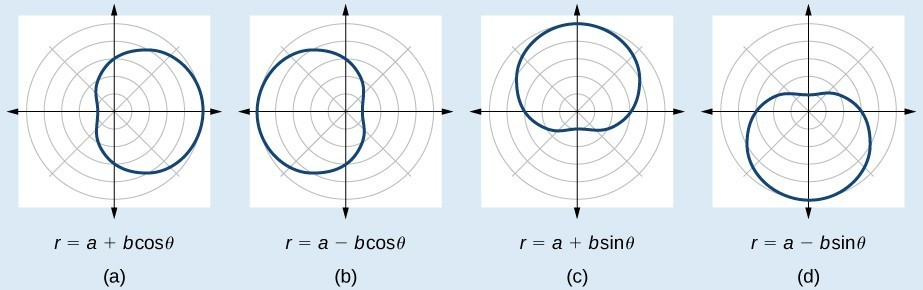
\includegraphics[width=0.7\textwidth]{limacon_polar}\\ \\
\textbf{Inner-loop Lima con}\\
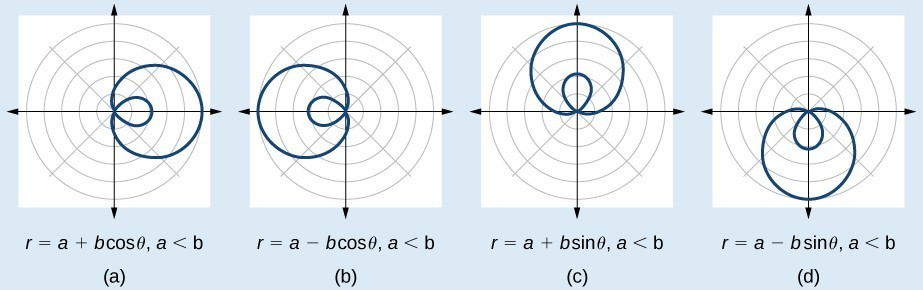
\includegraphics[width=0.7\textwidth]{limacon_inner_polar}
\subsection{Rose shape}
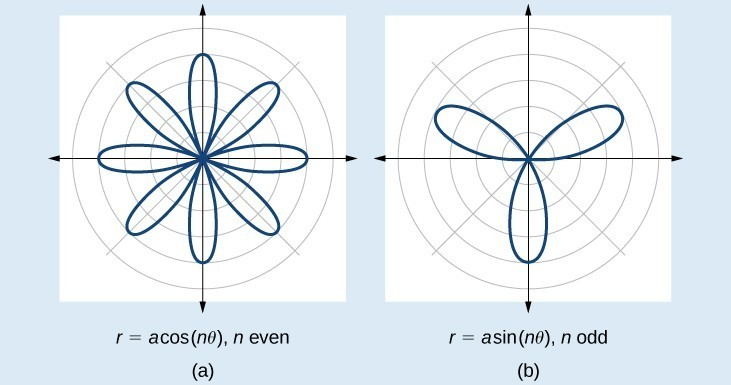
\includegraphics[width=0.35\textwidth]{rose_polar}\\
If $n$ is even the curve has $2n$ petals, if $n$ is odd the curve has $n$ petals

\subsection{Lemniscates shape}
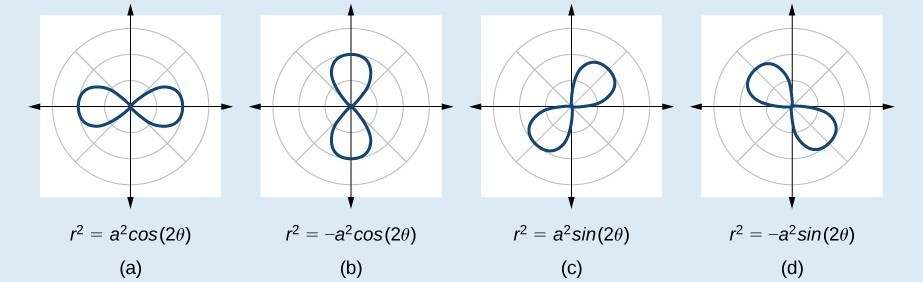
\includegraphics[width=0.7\textwidth]{lemniscates_polar}

\subsection{Spiral shape}
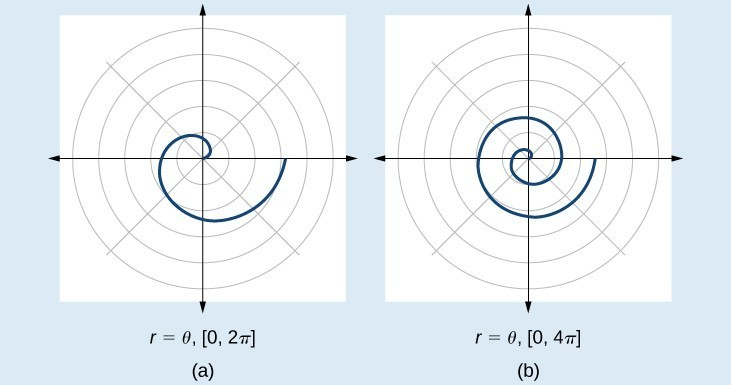
\includegraphics[width=0.35\textwidth]{spiral_polar}




\section{Finding area enclosed}
Area = $\dfrac{1}{2}\int_{\alpha}^{\beta} r^2d\theta$